\documentclass[utf8, 11pt]{feuille}

\newcommand{\titredutd}{\textbf{CC4 --- 2020}}

\begin{document}

\begin{center}
    \Large {\bf Contrôle continu}
    
    Lundi 17 décembre 2020 - durée: 2h30
\end{center}

Seules les calculatrices non communicantes et les notes manuscrites personnelles sont autorisées.

On rappelle les valeurs du nombre d'Avogadro ${\cal N_A}=6,02 \times 10^{23}$, de la constante de Boltzmann $k_B=1,38 \times 10^{-23}$ J.K$^{-1}$ et de leur produit, la constante des gaz parfaits $R=8,315$ J.K$^{-1}$ et de la constante de Planck réduite $\hbar = 1,05 \times 10^{-34}$ J.s.


% ______________________________________________________________________________
\section{L'hélium 3 à basse température}

On s'intéresse aux propriétés de l'hélium 3 ($^3$He) à basse température. $^3$He (masse molaire $M=3$ g.mol$^{-1}$ a un noyau
constitué de deux protons et d'un neutron et son spin, d'origine purement nucléaire, vaut $1/2$. Aux températures inférieures à 1 K, la solidification d'$^3$He est observée pour des pressions de l'ordre de 30 atm. Le but de ce problème est d'utiliser la physique statistique pour modéliser simplement les phases liquide et solide d'$^3$He à basse température et pour
interpréter une caractéristique surprenante du diagramme de phases connue sous le nom d'effet Pomerantchuk.

\subsection*{La phase liquide, gaz de fermions indépendants}

On modélise la phase liquide, volume $V$, température $T$ et potentiel chimique $\mu$ comme un \og gaz \fg \ de fermions indépendants de masse $m$ dont les niveaux
d'énergie  sont donnés par
\begin{align*}
\epsilon (k)=\Delta+\frac{\hbar^2 k^2}{2m}
\end{align*}
où $\Delta$ est une énergie constante traduisant la cohésion du liquide, et $k$ le vecteur d'onde.

\question
Comment s'appelle la statistique à laquelle obéissent les atomes d'$^3$He ? Rappeler l'expression du nombre moyen d'occupation $n(\epsilon)$ d'un micro-état d'énergie $\epsilon$.

\question
Montrer que la densité en énergie des micro-états s'écrit sous la forme $\rho (\epsilon)=A \sqrt{\epsilon-\Delta}$ où le calcul de $A$ fait appel à la quantification du vecteur d'onde dans la boîte de volume $V=L_xL_yL_z$. On utilisera des conditions aux limites périodiques pour exprimer les valeurs autorisées de $\vec{k}$.

\question
En déduire les expressions formelles du nombre moyen $\langle N \rangle$ de particules et de leur énergie moyenne $\langle E \rangle$ sous forme intégrale, en fonction de $T, V$ et $\mu$ et des données.

\question{Montrer qu'à température nulle $T=0$, tous les micro-états sont occupés jusqu'à un
niveau appelé \og niveau de Fermi\fg \ et caractérisé par un nombre d'onde $k_F$. Montrer que $k_F=\sqrt[3]{3\pi^2\frac{\langle N \rangle}{V}}$.}

\question
Expliquer pourquoi la pression et l'énergie cinétique du système ne sont pas nulles à $T = 0$.

\question
On donne le volume molaire d'$^3$He liquide : $v^L = 36$ cm$^3$.mol$^{-1}$. Calculer $k_F$ puis la vitesse caractéristique des atomes.

\question
On définit la température de Fermi par $k_BT_F =\frac{\hbar^2 k_F^2}{2m}$. Calculer numériquement $T_F$.
 
\question
Lorsque la température est non nulle mais faible devant  $T_F$, on montre que l'énergie cinétique moyenne du système s'écrit, à l'ordre le plus bas en $T/T_F$ comme
$$
\langle E_c \rangle=\frac{3}{5}\langle N \rangle k_B T_F \left[1+\left(\frac{5\pi^2}{12}\right) \left(\frac{T}{T_F}\right)^2+\ldots\right]
$$
Justifier qualitativement la dépendance observée en $T/T_F$ (on regardera ce qui peut se passer autour du niveau de Fermi).

\question
Exprimer l'énergie moyenne $\langle E \rangle$ en fonction de $\Delta$ et $\langle E_c \rangle$. En déduire la dépendance
de la capacité calorifique \textit{molaire} $C_V^L$ du liquide en fonction de $R$, $T$ et $T_F$.

On admettra pour la suite  que l'entropie \textit{molaire} du liquide est donnée par $S^L =C_V^L$.

\subsection*{Modélisation de la phase solide}

Dans le solide, les atomes d'$^3$He sont localisés sur leurs sites. On distingue alors deux
contributions aux propriétés thermodynamiques du solide à basse température : (1) celle
des $N$ spins $1/2$ localisés et supposés indépendants et (2) celle des vibrations du réseau
cristallin dont les modes constituent un gaz parfait de bosons, appelés \og phonons\fg.

\question
Calculer la contribution des spins à l'entropie totale du solide. On pourra se placer dans l'ensemble canonique en remarquant que le champ magnétique extérieur est nul et que tous les micro-états de spins ont une énergie nulle à toute température. Cette contribution est-elle nulle à $T = 0$ ?

\question
Les phonons sont des bosons en nombre non fixé. Comment s'appelle la statistique à laquelle ils obéissent ? Donner l'expression du nombre moyen d'occupation d'un micro-état d'énergie $\epsilon$.

On admet que l'entropie molaire des phonons s'exprime à basse température ($T \ll T_D$) comme
$$
S^p=\frac{4\pi^4}{5} R \left(\frac{T}{T_D}\right)^3
$$
$T_D$, la température de Debye, définie par $k_B T_D=\hbar c_s \sqrt[3]{6\pi^2 \frac{{\cal N}_A }{V}}$ ($c_s$ est la vitesse du son dans le solide).

\question
Donner l'expression littérale de l'entropie molaire totale du solide dans cette limite (en incluant la
contribution des spins).

\question
Montrer que pour $T \simeq 0,1$ K, la contribution des phonons à l'entropie du solide est
négligeable devant celle des spins. On calculera la température de Debye. On donne $c_s=300$ m.s$^{-1}$ et le volume molaire du solide $v^s = 24$ cm$^3$.mol$^{-1}$.

\subsection*{l'effet Pomerantchuk}


\begin{center}\scalebox{1.1}{
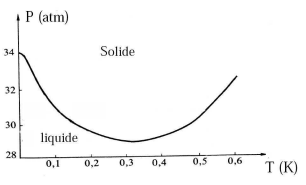
\includegraphics{Pom.png}} \\
\textit{Courbe de fusion dans le plan ($T, p$) pour l'hélium 3 à basse température.}
\label{Pom}
\end{center}

La figure (\ref{Pom}) montre la courbe de coexistence solide-liquide à basse température dans le plan température-pression.

\question
Quel phénomène a priori paradoxal observe-t-on pour $T < 0,32$ K ? Ce phénomène, prévu théoriquement en 1950, est appelé \og effet Pomerantchuk\fg.

\question
Sommes nous dans un domaine de températures où on peut utiliser les résultats des parties précédentes ?

On rappelle la relation de Clausius-Clapeyron le long de la courbe de fusion: $\frac{dp}{dT}\vert_{fusion}=\frac{S^L-S^s}{v^L-v^s}$ où $S^L$, $S^s$, $v^L$ et $v^s$ sont les entropies et volumes molaires des deux phases.

\question
Montrer que nos modélisations des phases liquide et solide d'$^3$He permettent d'expliquer l'effet
Pomerantchuk. Montrer  que ce modèle prévoit un comportement habituel de la courbe de coexistence au-dessus d'une certaine température que l'on exprimera en fonction de $T_F$ . Estimer numériquement cette température et comparer à la figure (\ref{Pom}).



% ______________________________________________________________________________
\section{Mélange binaire en phase liquide}

Le but de ce problème est d'étudier un modèle simple du mélange de deux corps purs
liquides, dit \og modèle des solutions régulières\fg. Le système est constitué de $N_1$ particules de \og liquide 1\fg \ et de $N_2$ particules de \og liquide 2 \fg \ placées dans un volume $V$ constant en contact avec un thermostat à la température $T$. Les deux liquides ne sont pas susceptibles de réagir chimiquement de sorte que $N_1$ et $N_2$ sont fixés.

\subsection*{Mise en jambe}

\question
Dans quel ensemble statistique le choix des variables $T$, $V$ , $N_1$ et $N_2$ place-t-il implicitement l'étude ?

\question
On suppose que les deux liquides sont incompressibles et que les volumes par particule dans chaque liquide pur, notés $v_1(T)$ et $v_2(T)$, sont inchangés dans le mélange. Montrer alors que les seules trois variables T, $N_1$ et $N_2$ suffisent à l'étude du mélange.

\question
On suppose de plus que $v_1(T) \simeq v_2(T)$ de sorte qu'il est raisonnable de placer les molécules sur un réseau constitué de $N=N_1+N_2$ sites de même volume comme l'illustre la figure (\ref{MB}) ci-dessous. Exprimer le nombre total $\Omega(N_1, N_2)$ de configurations microscopiques accessibles au système.



\begin{center}\scalebox{0.6}{
\includegraphics{Melangebinaire4.png}} \\
\textit{Modèle d'un mélange binaire sur un réseau carré avec $N_1=7$ et $N_2=9$.}
\label{MB}
\end{center}


\subsection*{Modélisation des interactions}

Dans un liquide, l'énergie d'interaction entre particules constitue le terme dominant dans l'expression de l'énergie d'un micro-état. Ces interactions ayant une faible portée, on se limite aux interactions entre une particule donnée et les $q$ particules \og plus proches voisines \fg \ (ppv). Dans le cas d'un réseau carré, on a $q = 4$. On introduit alors trois termes d'interaction $u_{11}, u_{22}$ et $u_{12}$ correspondant respectivement aux énergies d'interaction entre paires de particules ppv 1-1, 2-2 et 1-2. Dans une configuration des particules données (un micro-état), on désigne par $N_{11}, N_{22}$ et $N_{12}$ respectivement les nombres de paires de particules ppv 1-1, 2-2 et 1-2.

\question
Que valent $N_{11}, N_{22}$ et $N_{12}$ dans l'exemple de la figure (\ref{MB}) ? Montrer (sur un exemple) qu'avec une autre configuration des particules, ces nombres changent.

\question
Exprimer l'énergie d'un micro-état en fonction de $N_{11}, N_{22}$, $N_{12}$, $u_{11}, u_{22}$ et $u_{12}$.

\question
\`A la limite thermodynamique, on peut négliger l'effet des bords du réseau. En considérant d'abord les particules de liquide 1, montrer que $q N_1$ est relié de façon simple à $N_{11}$ et  $N_{12}$. Trouver de même la relation entre $q N_2$, $N_{22}$ et  $N_{12}$.

\question
En déduire que l'énergie d'un micro-état n'est fonction que de $N_1, N_2$ et $N_{12}$ et qu'elle s'écrit
$$
E(N_1, N_2, N_{12})= \frac{q}{2} N_1 u_{11}+\frac{q}{2} N_2 u_{22}+N_{12}(u_{12}-\frac{u_{11}+ u_{22}}{2})
$$

Dans la suite, on posera $u=u_{12}-\frac{u_{11}+ u_{22}}{2}$.

\question
On introduit le nombre $\omega(N_1, N_2, N_{12})$ de micro-états du système contenant $N_{12}$ paires de particules ppv 1-2. Quelle relation formelle lie $\Omega(N_1, N_2)$ et $\omega(N_1, N_2, N_{12})$ ? On ne cherchera pas à calculer $\omega(N_1, N_2, N_{12})$.

\question
Exprimer la fonction de partition $Z(T, N_1, N_2)$ du système comme une somme sur $N_{12}$
 faisant intervenir $\omega(N_1, N_2, N_{12})$ et $E(N_1, N_2, N_{12})$.

\subsection*{Approximation de champ moyen}

Le nombre $\omega(N_1, N_2, N_{12})$ n'étant pas calculable analytiquement, l'expression de $Z$
trouvée à la question précédente est inutilisable. On propose donc l'approximation suivante: $N_{12}=qp_1p_2(N_1 + N_2$) où $p_1$ et $p_2$ sont les probabilités qu'un site soit occupé par une particule de liquide 1 et 2 respectivement.

\question
On introduit la fraction molaire $\phi$ en particules de liquide 1 définie par $\phi=\frac{N_1}{N_1+N_2}$. Exprimer $p_1$ et $p_2$ en fonction de $\phi$.

\question
Proposer une interprétation simple de l'expression approchée de $N_{12}$. Justifier l'appellation d'approximation de \og champ moyen\fg .

\question
En déduire l'expression de l'énergie d'un micro-état $E=E(N_1, N_2)$ dans l'approximation de champ moyen en fonction de $N, q, \phi$ et des énergies $u_{11}, u_{22}$ et $u_{12}$.

\question
Montrer alors que la fonction de partition du système s'écrit simplement en fonction de $\Omega(N_1, N_2)$ et de $E(N_1, N_2)$.

\question
Calculer enfin l'énergie libre $F(T,N_1,N_2)$ du système. On utilisera la formule de Stirling pour exprimer $\ln ( \Omega)$ et on montrera que
\begin{align*}
F(T,N_1,N_2)&=(N_1+N_2)f(T,\phi)\\
f(T,\phi)&=\frac{qu_{11}}{2} \phi +\frac{qu_{22}}{2} (1-\phi) +q u \phi(1-\phi)+k_BT \left[ \phi \ln (\phi)+(1-\phi) \ln (1-\phi) \right]
\end{align*}

\subsection*{Diagramme de phases du mélange}

On admet que le mélange binaire 1+2 est stable si et seulement si $\left(\frac{\partial^2f}{\partial \phi^2}\right)_T >0$.

\question
Calculer $\left(\frac{\partial^2f}{\partial \phi^2}\right)_T$ pour étudier la concavité de $f(T,\phi)$.

\question
Montrer que si $u \le 0$, le mélange est stable.

\question
Montrer que si $u > 0$, il existe une température critique $T_C$ séparant deux régimes distincts. En raisonnant par analogie avec la transition gaz-liquide, décrire ce qui se passe lorsque $T < T_C$. Donner l'équation de la courbe spinodale, c'est-à-dire le lieu des points où $\left(\frac{\partial^2f}{\partial \phi^2}\right)_T=0$. On pourra poser $\phi=\frac{1+\alpha}{2}$ avec $-1 \le \alpha \le 1$ et calculer $\alpha (T)$ sur la spinodale.

\question
Proposer une interprétation physique du signe de $u$ permettant d'expliquer qualitativement les résultats précédents.


\begin{center}\scalebox{0.7}{
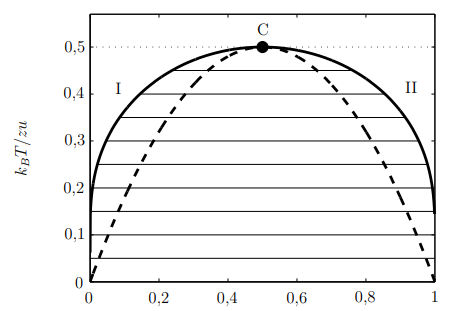
\includegraphics{DiagrammePhaseMB.png}} \\
\textit{Diagramme de phases pour le modèle des solutions régulières avec $u > 0$. La courbe en pointillée est la spinodale, la courbe pleine est la courbe de coexistence liquide-liquide.}
\label{DPMB}
\end{center}




\end{document}


